%(BEGIN_QUESTION)
% Copyright 2009, Tony R. Kuphaldt, released under the Creative Commons Attribution License (v 1.0)
% This means you may do almost anything with this work of mine, so long as you give me proper credit

An NDIR gas analyzer is going to be used to measure the concentration of carbon monoxide (CO) in ``synthesis gas'' produced by a biomass gasification process.  This process converts dry organic matter into a flammable gas stream which may be used to run an internal combustion engine:

$$\includegraphics[width=15.5cm]{i04173x02.eps}$$

Other gases known to be in this stream in large quantity include nitrogen (N$_{2}$) and hydrogen (H$_{2}$).  The infrared absorption characteristics of carbon monoxide are shown in the following plot.  Neither nitrogen nor hydrogen gas absorbs infrared light to any appreciable degree:

$$\includegraphics[width=15.5cm]{i04173x01.eps}$$

Identify which gases the ``reference cell'' and ``detector'' chambers of the NDIR analyzer should be filled with, and whether or not this analyzer will require filter cells.  If filter cells are required, identify the gas(es) they should be filled with as well.

\vskip 20pt \vbox{\hrule \hbox{\strut \vrule{} {\bf Suggestions for Socratic discussion} \vrule} \hrule}

\begin{itemize}
\item{} Explain why the differential pressure transmitter has its {\it low-pressure} port connected to the gasifier (with the high-pressure port vented), rather than the other way around.
\item{} A gasifier's operation should be such that the production of flammable gases such as H$_{2}$ and CO are maximized.  Explain how too much air admitted into the gasifier would cause a decrease in production of these fuel gases.
\end{itemize}

\underbar{file i04173}
%(END_QUESTION)





%(BEGIN_ANSWER)


%(END_ANSWER)





%(BEGIN_NOTES)

Fill the detector chambers with carbon monoxide (CO) gas.  Fill the reference cell with any non-absorbing gas (e.g. nitrogen).

\vskip 10pt

So long as no other light-absorbing gases are present in the synthesis gas, no gas-filled Luft detectors are required for this analyzer.  If carbon monoxide is the only gas in the process stream capable of absorbing infrared light, then there are no interfering species.

%INDEX% Measurement, analytical: nondispersive optical
%INDEX% Process: biomass gasification (downdraft gasifier)

%(END_NOTES)


